\begin{figure}[ht!]
    \centering
    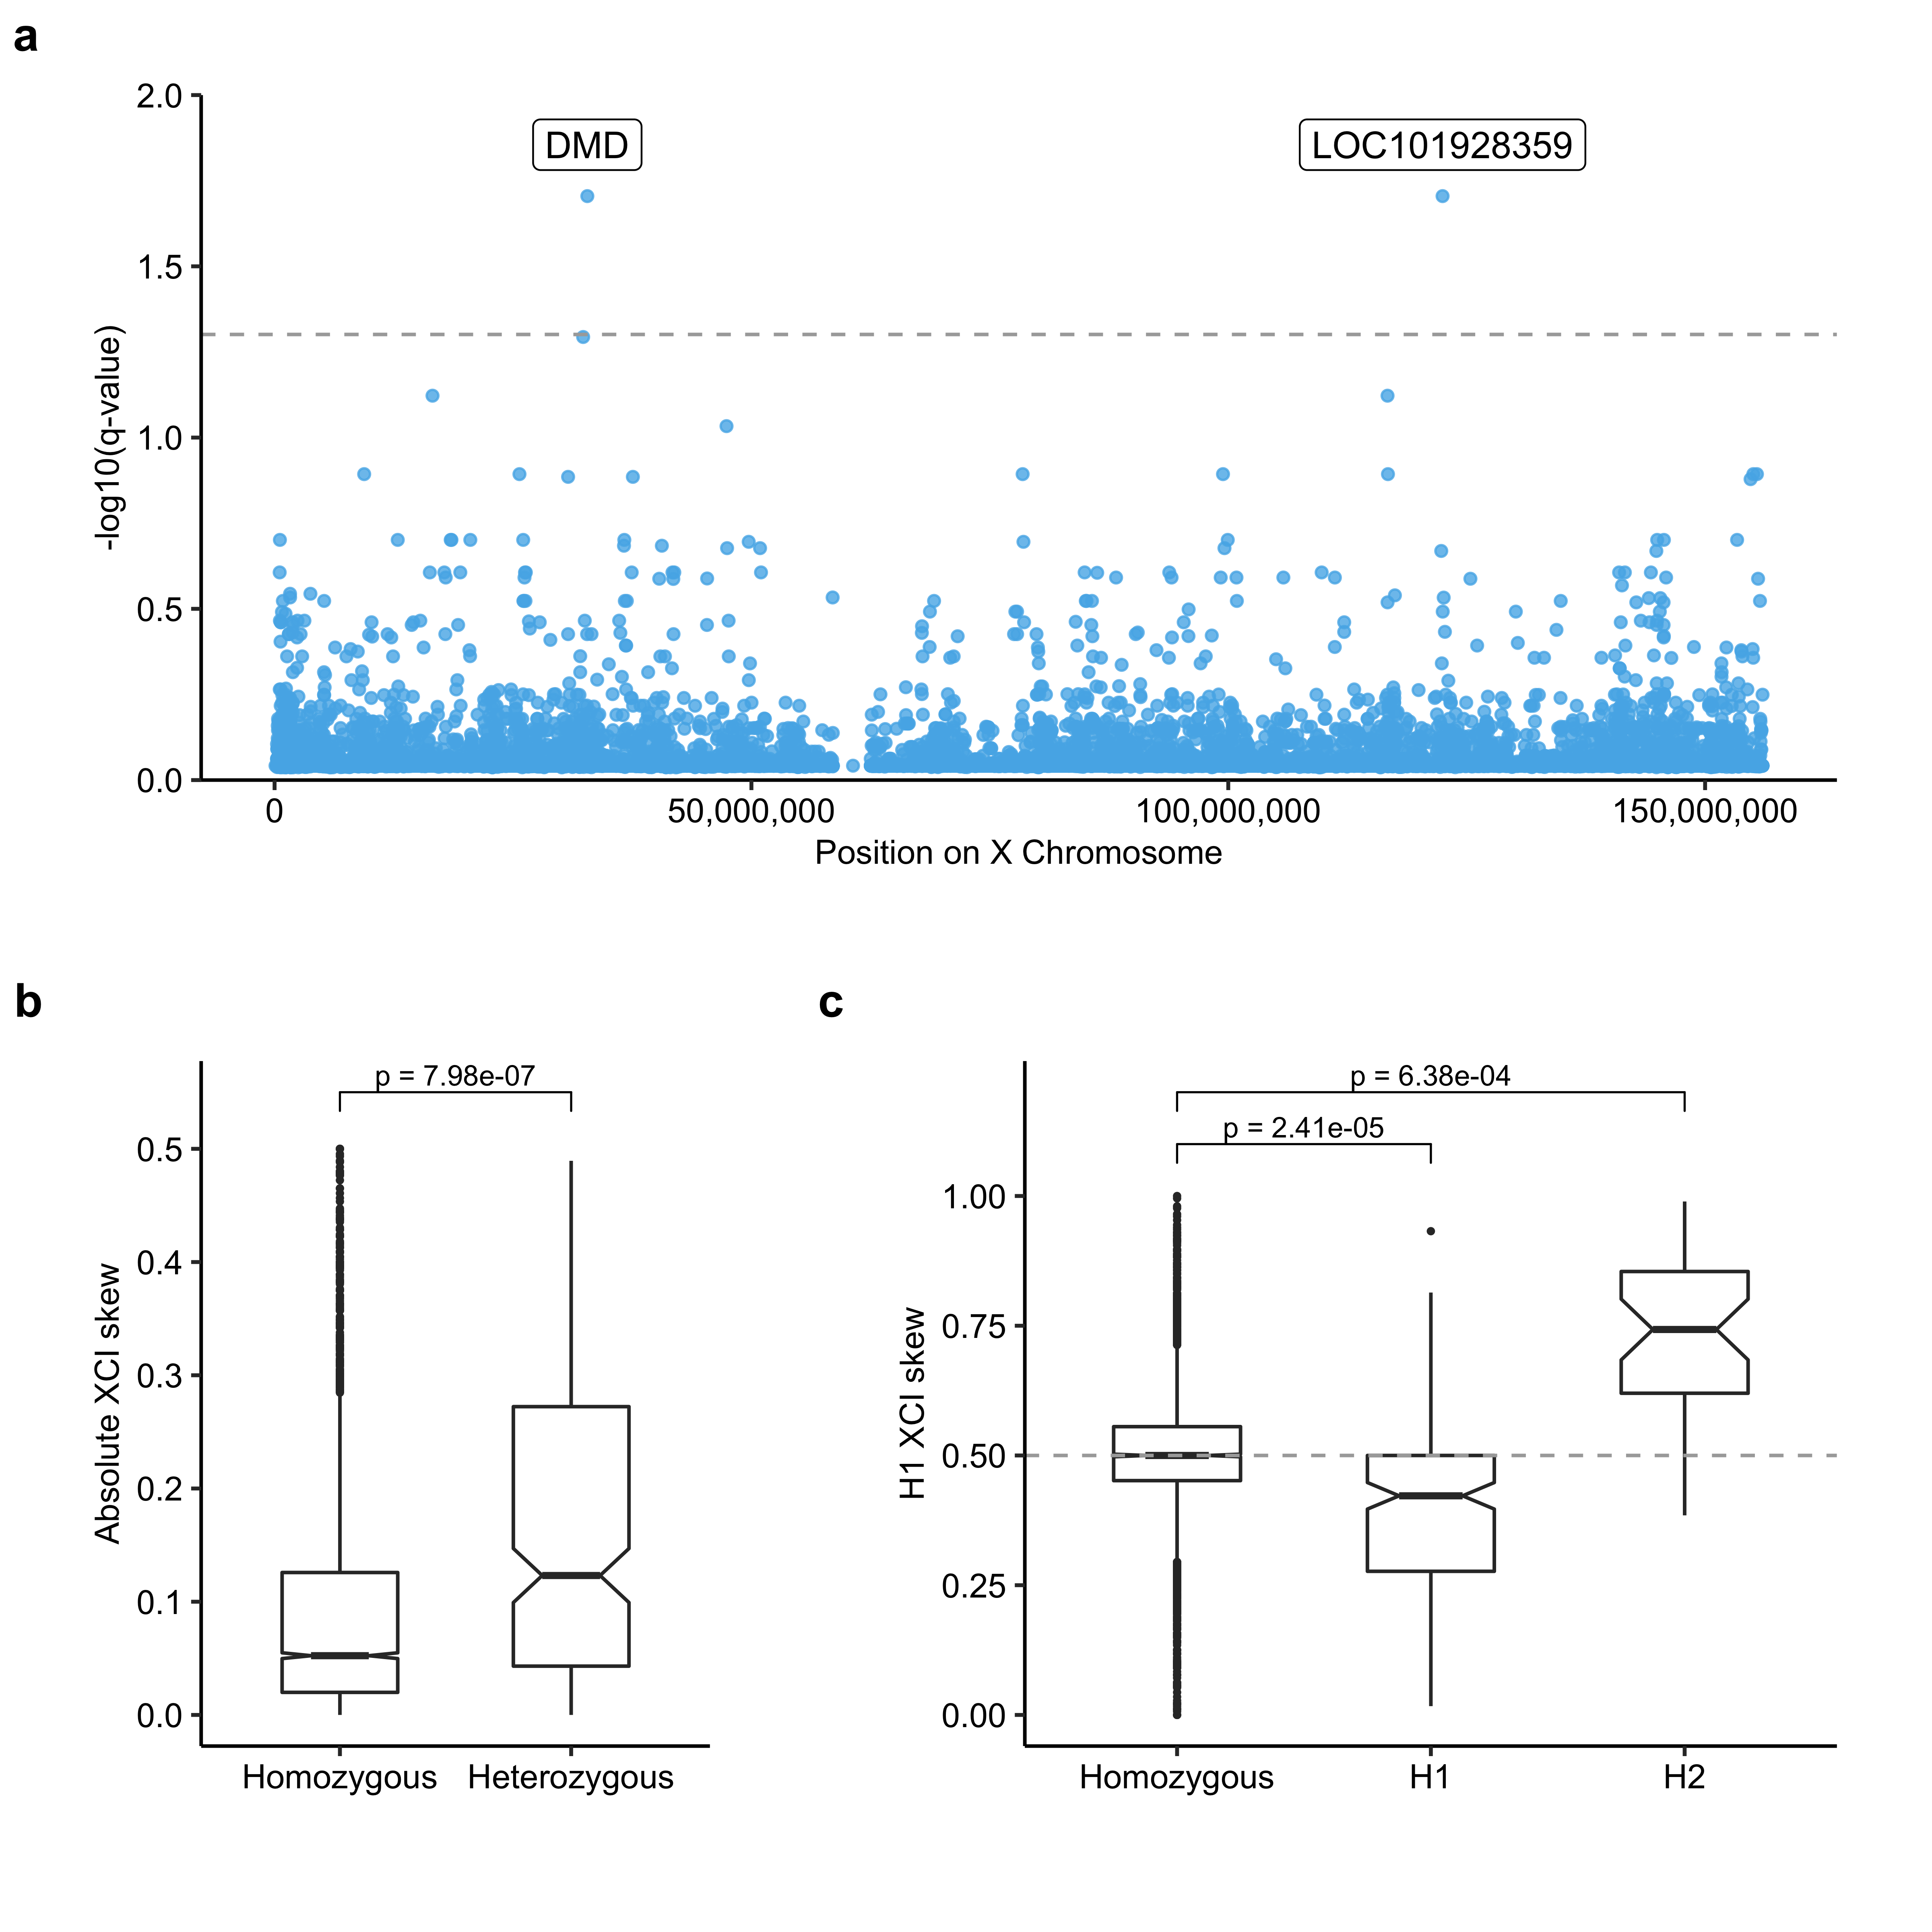
\includegraphics[width=0.75\textwidth]{chapter4/Figures/Figure_3.png}
    \caption{
        Associating specific variation on the X chromosome with inactivation skew. 
        \textbf{a}, Manhattan plot of -log10(q-values) generated from a linear mixed model associating absolute XCI skew with heterozygous status, accounting for age as well as individual and tissue groupings of samples. A one-sided test was performed under the hypothesis that heterozygous status increases absolute skew. Dotted horizontal line indicates local false discovery rate of 0.05. 
        \textbf{b}, Boxplot of absolute XCI skew in samples that are homozygous  (n = 4,232) or heterozygous (n = 230) for the DMD variant (rs141680486). Indicated p-value is from the model described above.
        \textbf{c}, Boxplot of skewing toward haplotype 1 (H1), where the grouping on the x-axis describes individuals without the DMD variant (Homozygous, n = 4,232), with the variant on haplotype 1 (H1, n = 190), and with the variant on haplotype 2 (H2, n = 40). Indicated p-values are from the model described above but with a two-sided test, since we do not assume the direction of skewing associated with a specific variant.}
    \label{fig:fig4.3}
\end{figure}